\documentclass[]{ctexart}
\usepackage{amsmath,graphicx,textcomp,subfigure,indentfirst,ctex,color,float}
\usepackage{xcolor}

\title{Lecture2}
\date{\today}
\newcommand{\new}[1]{\textcolor{blue}{#1}}
\begin{document}
\maketitle

% \section*{回顾}

% 宇宙大爆炸理论的经典证据:
% \begin{itemize}
% 	\item 哈勃图
%     \item 微波背景辐射
%     \item 原初核合成
% \end{itemize}

% \section{宇宙成分组成}

% \begin{itemize}
% 	\item 恒星、星系 $\sim$0.5\%
%     \item 气体(星际介质、星系际介质) $\sim$4\%
%     \item 光(radiation)$\sim$0.05\%, 宇宙早期重要组分
%     \item 中微子 $\sim$0.5\%
%     \item 暗物质 $\sim$25\%
%     \item 暗能量 $\sim$70\%,主导宇宙加速膨胀
% \end{itemize}

% \subsection{暗物质}

% \par 暗物质:参加引力相互作用,不参加电磁相互作用的一种物质,很可能是超出粒子物理标准模型的新粒子。

% 暗物质存在的证据:
% \begin{itemize}
% 	\item 星系旋转曲线:星系外侧的旋转速度高于可见物质预测的旋转速度。(21厘米线测量星系外侧的速度。)
%     \item 子弹星系团:两个星系碰撞,强引力透镜测量引力中心,X射线测量重子物质中心,发现二者分离。
%     \item CMB支持 $\Lambda$CDM 模型。(其中 $\Lambda$ 表示暗能量的模型“宇宙学常数”,CDM是冷暗物质 cold dark matter 的缩写。)
%     \item 大尺度结构形成:在今天的宇宙年龄这段时间中,重子物质密度不足以形成如今的大尺度结构——大尺度结构实际上由暗物质主导形成。
% \end{itemize}

% \subsection{暗能量}

% 暗能量存在的证据:
% \begin{itemize}
% 	\item Ia型超新星测量到宇宙的加速膨胀,支持 $\Lambda$CDM 模型。
%     \item CMB支持 $\Lambda$CDM 模型。
% \end{itemize}

\section*{宇宙学基础}

\section{宇宙学原理}

宇宙物质在空间分布上是均匀 (Homogeneous) 和各向同性的 (Isotropic)。

\begin{itemize}
	\item Isotropic推不出Homogeneous。
    \item “哥白尼原理”:宇宙中不存在任何一个“特殊”的观测者。
    \item Isotropic加上“哥白尼原理”可以得到Homogeneous。因为对于宇宙中任意两点,我们都能找到一个观测者和两点等距。根据各向同性,可以推出这两点的物质密度相同。
    % \item Homogeneous推不出Isotropic。Homogeneous加上“哥白尼原理”可以得到Isotropic。
\end{itemize}

\subsection{检验物质分布的均匀性}
在宇观尺度(尺度越大,均匀性越好),
我们把宇宙平均密度表示为 $\bar{\rho}$,
根据均匀性原理,包含在球体 $R$ 内的平均质量 $M=\bar{\rho}\times\frac{4}{3} \pi R^3$。
实际上,由于宇宙中物质密度分布存在涨落,实际 球体 $R$ 内的质量为$M+\Delta M$ 。
质量涨落的平均值 $\left\langle \Delta M \right\rangle = 0$,方均根 $\sqrt{ \left\langle \Delta M \right\rangle ^2 } = \delta M$。
定义$\sigma (M) = \frac{\delta M}{M}$,当$\sigma (M) > 1$,宇宙在对应的$R$尺度上是不均匀的。

观测发现 $\sigma_8 \equiv \sigma(R=8 h^{-1} \mathrm{~Mpc} ) \simeq 0.8$ ,说明$8 h^{-1} \mathrm{~Mpc}$大致是线性尺度与非线性尺度的分水岭。
其中 $h \equiv H_0 / (100 \mathrm{~km~s^{-1}~Mpc^{-1}}) \simeq 0.7$,$H_0$是哈勃常数。
$\sigma(M)=\sigma_{8}\left(\frac{M}{M_{8}}\right)^{-(3+n) / 6}$,其中$n\simeq 0.97$,估算出$\sigma(R=100 h^{-1} \mathrm{~Mpc} ) \simeq 0.005$,所以在$R \ge 100 h^{-1}\mathrm{~Mpc}$ 可以认为宇宙是均匀的。

\subsection{检验物质分布各向同性}

宇宙微波背景辐射(CMB)温度 $T (\hat{n}) = \bar{T} + \Delta T (\hat{n})$ , 其中 $\hat{n}$ 是某一方向的单位向量, $\bar{T}$ 是平均温度。
根据定义,CMB温度涨落的平均值$\left\langle \Delta T (\hat{n}) \right\rangle = 0$ 。
我们定义 $\delta T \equiv \sqrt{\left\langle \Delta T^2 (\hat{n}) \right\rangle}$  ,测量到CMB的温度涨落 $\frac{\delta T}{T} \simeq 10^{-5}$ ,
是对各向同性的足够好的检验。

\section{哈勃定律 Hubble's Law}

哈勃测量到遥远天体(不受引力束缚)的退行速度 $v=H_0 R$ ,其中 $H_0$ 是哈勃常数。定义红移 $z=\frac{v}{c}$ ,其中 $v \ll c$ 。 

哈勃定律并不代表我们是“特殊”的观测者,因为宇宙中其它位置的观测者一样会观测到哈勃定律。
\begin{figure}[!hbtp]
    \centering
    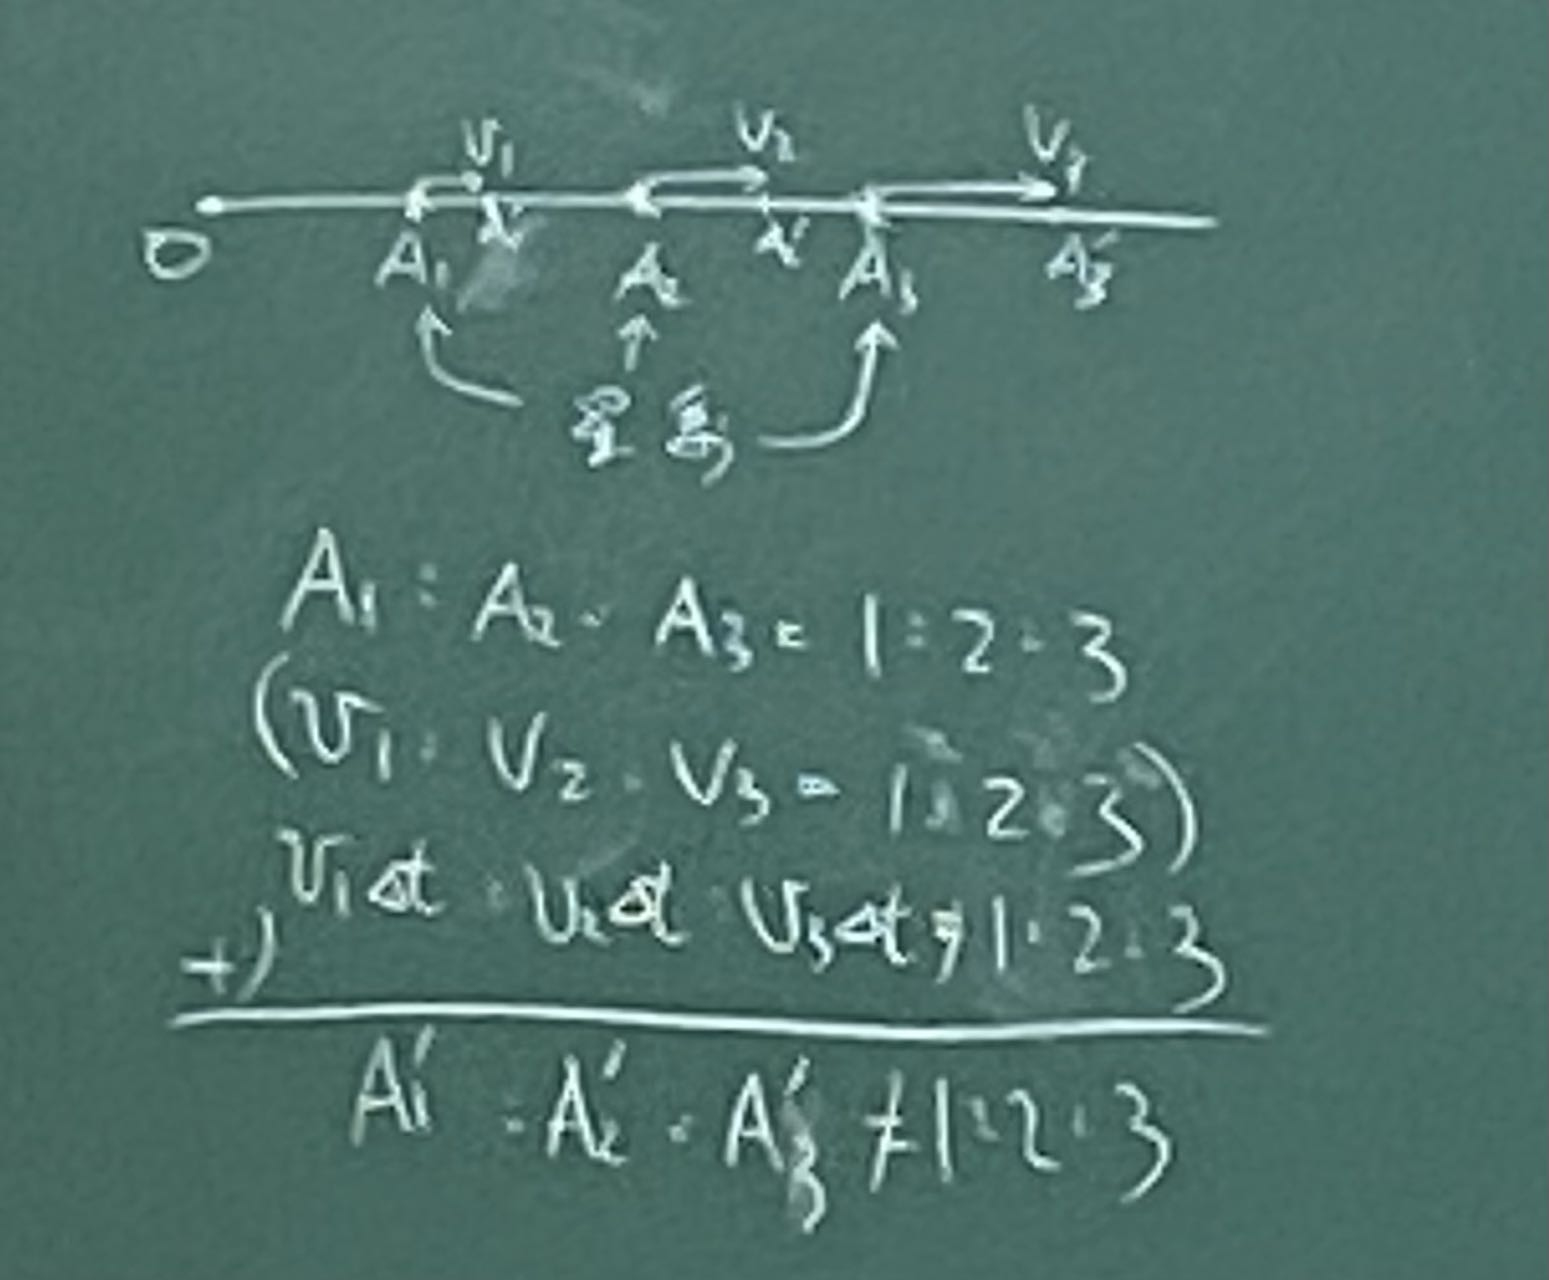
\includegraphics[width=0.5\textwidth]{figures/Hubble.jpg}
    \caption{其它位置的观测者一样会观测到哈勃定律}
\end{figure}


考虑到和宇宙学原理自洽,哈勃定律可以解释为宇宙(准确的来说是“时空”)在均匀膨胀。

\subsection{尺度因子}

对于给定观测者,某一遥远天体的位置随着时间变化 $\vec{x}(t) = \vec{x} (t_0) \frac{a(t)}{a(t_0)}$,
定义$a(t)$为尺度因子,尺度因子刻画宇宙整体的膨胀,是时间的函数,与位置无关(符合宇宙学原理的“均匀性”)。
\begin{figure}[!hbtp]
    \centering
    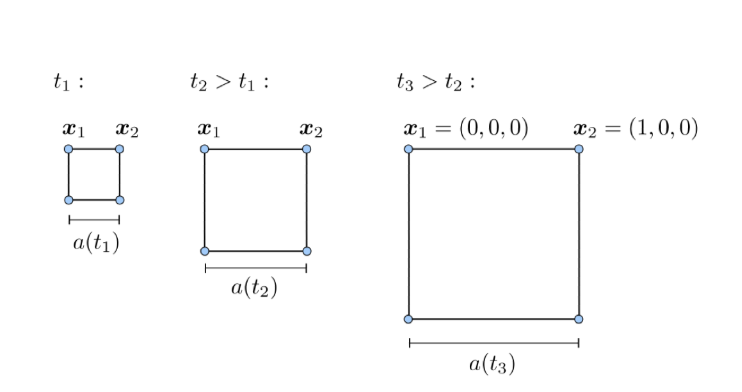
\includegraphics[width=0.8\textwidth]{figures/scale_factor.png}
    \caption{尺度因子 $a(t)$,图源Dodelson}
    \label{fig:scale_factor}
\end{figure}
$t_0$ 时刻,物理长度=坐标长度。

\subsection{哈勃参数}

从宇宙膨胀可以推出哈勃定律。
遥远天体的退行速度
\begin{equation}
    \begin{aligned} \vec{v}(t)=\frac{d \vec{x}}{d t} &=x\left(t_{0}\right) \frac{1}{a\left(t_{0}\right)} d a / d t \\ &=x\left(t_{0}\right) \frac{a(t)}{a\left(t_{0}\right)} \frac{d a / d t}{a(t)} \end{aligned}
\end{equation}

定义哈勃参数 $H(t) \equiv \frac{da/dt}{a} = \frac{\dot{a}}{a}$,可以得到哈勃定律 $\vec{V}(t)=\vec{x}(t)H(t)$,所以 $H_0$ 就是今天的哈勃参数。


因为历史原因, $H_0 = 100 h \mathrm{~km} \mathrm{~s}^{-1} \mathrm{~Mpc}^{-1}$ , $h \simeq 0.7$.

今天更精确的测量出现 Hubble tension 问题,CMB的测量给出的结果是0.67,SN Ia的测量给出的结果是0.74,对标准宇宙学模型$\Lambda$CDM提出了挑战。

\subsection{讨论}
根据 $z=\frac{v}{c}=c^{-1} H_0 R$,当$R>c H_0^{-1}$时,似乎有 $z>1$ 且 $v>c$ ……

\begin{itemize}
    \item 有没有红移大于1的天体?——有。
    \item 红移大于1的天体是否超过光速?
    \begin{itemize}
        \item 相对论下的多普勒红移:当 $z\gg 1$,$v\rightarrow c$时, $z=\sqrt{\frac{1+v/c}{1-v/c}}-1$ 
        \item 但哈勃观测到的红移实际上并不能用多普勒红移解释。多普勒红移适用于平直时空,而哈勃定律是时空整体的膨胀。
        \item 在宇宙学的尺度下,可测量量不是速度而是红移。$z=\frac{v}{c}$只适用于本地。在高红移处需要另外寻找红移和距离的关系$z=z(R)$
        \item 定义哈勃流(Hubble flow)的“速度” $\vec{V}_H(t)=H(t) \vec{R}(t)$,它只是为了方便表达定义出的速度,而不是直接可测量的物理量。膨胀的宇宙是弯曲时空,而在弯曲时空里,只有本地惯性参考系里定义的速度才是可测量的物理量。相对地有“本动速度”(天体相对于哈勃流的速度) $\vec{v}_\text{pec}$,总体的速度为两者之和 $\vec{V} = H\vec{R}+\vec{v}_\text{pec}$ ,可以大于光速,但这并不是物理上的速度。
    \end{itemize}
    \item 红移大于1的天体会超出视界吗?——不会。应该使用$z=z(R)$计算。
\end{itemize}

\end{document}
